% Historical reference. The active design is Figure 1 in agentic.pdf.
\documentclass[11pt,a4paper]{article}

% --- Core Geometry and Typography ---
\usepackage[utf8]{inputenc}
\usepackage[T1]{fontenc}
\usepackage{lmodern}
\usepackage[margin=1in]{geometry}
\usepackage{amsmath,amssymb,amsfonts}
\usepackage{microtype}
\usepackage{booktabs}
\usepackage{tabularx}
\usepackage{xcolor}
\usepackage{hyperref}
\usepackage{listings}
\usepackage{enumitem}

% --- TikZ and Diagram Libraries ---
\usepackage{tikz}
\usetikzlibrary{
    shapes.geometric,
    arrows.meta,
    positioning,
    fit,
    calc,
    backgrounds,
    shadows.blur,
    decorations.pathreplacing
}

% --- Custom Colors ---
\definecolor{trinPrimary}{RGB}{18, 52, 86}      % Navy Deep
\definecolor{trinSecondary}{RGB}{41, 128, 185}  % Cerulean
\definecolor{trinAccent}{RGB}{231, 76, 60}      % Crimson Hold
\definecolor{trinWarn}{RGB}{243, 156, 18}       % Amber Step-up
\definecolor{trinSuccess}{RGB}{39, 174, 96}     % Emerald Allow
\definecolor{trinPurple}{RGB}{142, 68, 173}     % SOC Purple
\definecolor{trinDark}{RGB}{33, 37, 41}         % Slate Dark
\definecolor{trinLight}{RGB}{248, 249, 250}     % Off-White
\definecolor{trinBoxBg}{RGB}{240, 244, 248}     % Soft Blue Grey

% --- Hyperref Setup ---
\hypersetup{
    colorlinks=true,
    linkcolor=trinSecondary,
    citecolor=trinPrimary,
    urlcolor=trinSecondary,
    pdftitle={TRINETRA: Diagrammatic System Design and Architectural Workflow},
    pdfauthor={TRINETRA Engineering Team}
}

% --- TikZ Style Definitions ---
\tikzset{
    baseBox/.style={
        rectangle,
        rounded corners=4pt,
        draw=trinPrimary!80,
        fill=white,
        line width=1pt,
        align=center,
        font=\small\sffamily,
        blur shadow={shadow blur steps=3, shadow xshift=1pt, shadow yshift=-1pt, shadow opacity=20}
    },
    ingestBox/.style={
        baseBox,
        draw=trinSecondary!90,
        fill=trinSecondary!8,
        minimum width=3.4cm,
        minimum height=1.1cm
    },
    engineBox/.style={
        baseBox,
        draw=trinPrimary,
        fill=trinBoxBg,
        minimum width=3.8cm,
        minimum height=1.3cm
    },
    policyBox/.style={
        baseBox,
        draw=trinPrimary!90,
        fill=trinPrimary!10,
        line width=1.4pt,
        minimum width=11.5cm,
        minimum height=1.4cm
    },
    decisionBox/.style={
        baseBox,
        minimum width=3.2cm,
        minimum height=1.1cm,
        font=\small\bfseries\sffamily
    },
    allowBox/.style={decisionBox, draw=trinSuccess, fill=trinSuccess!12, text=trinSuccess!80!black},
    warnBox/.style={decisionBox, draw=trinWarn, fill=trinWarn!15, text=trinWarn!80!black},
    holdBox/.style={decisionBox, draw=trinAccent, fill=trinAccent!15, text=trinAccent!90!black},
    socBox/.style={
        baseBox,
        draw=trinPurple,
        fill=trinPurple!10,
        text=trinPurple!80!black,
        minimum width=4.5cm,
        minimum height=1.2cm
    },
    flowArrow/.style={
        -{Stealth[scale=1.1]},
        line width=1.1pt,
        draw=trinDark!80
    },
    dashArrow/.style={
        -{Stealth[scale=1.1]},
        line width=1pt,
        dashed,
        draw=trinSecondary!90
    },
    alertArrow/.style={
        -{Stealth[scale=1.2]},
        line width=1.3pt,
        draw=trinAccent
    },
    groupFrame/.style={
        draw=black!25,
        fill=black!2,
        rounded corners=6pt,
        dashed,
        inner sep=10pt
    }
}

\title{
    \vspace{-1.5cm}
    \textbf{\LARGE TRINETRA: Technical System Design \& Architectural Workflow}\\[0.3em]
    \large Pre-Settlement In-Line Interception of Generative AI Cyber Fraud and Multi-Hop Mule Networks
}
\author{\textbf{System Engineering \& Security Architecture Specification}}
\date{\today}

\begin{document}

\maketitle

\begin{abstract}
This technical specification articulates the end-to-end system design, modular data flows, and sub-150ms execution lifecycle of \textbf{TRINETRA} (\textit{The Third Eye of Digital Trust}). Built to counter next-generation financial cybercrime, TRINETRA unifies three real-time analytic engines: (i) an acoustic digital signal processing (DSP) voice clone forensics module, (ii) an in-memory directed graph topology engine for 5-hop mule ring and cycle identification, and (iii) a compiled regular expression Natural Language Processing (NLP) taxonomy for extortion and ``digital arrest'' coercion detection. We detail the system's component layout, message schemas, mathematical decision bounds, fail-safe override gating, and real-time WebSocket telemetry pipeline via formal architectural diagrams.
\end{abstract}

\tableofcontents
\vspace{0.8em}
\hrule
\vspace{1em}

% =========================================================================
\section{System Overview \& Operational Objectives}
\label{sec:overview}
% =========================================================================

Conventional fraud detection infrastructures (e.g., legacy rule engines and asynchronous anti-money laundering monitors) evaluate transactions \textit{post-settlement} using relational tabular heuristics. In modern generative AI fraud, authentic credentials are legitimately submitted by victims under synthetic coercion, rendering conventional credential checks and static rules obsolete.

TRINETRA introduces a pre-settlement, in-line security middleware operating at the bank payment gateway boundary. Its design satisfies four technical requirements:
\begin{enumerate}[leftmargin=1.8em, itemsep=2pt]
    \item \textbf{Sub-150ms Decision SLA:} Complete end-to-end feature extraction, multi-vector graph traversal, and policy scoring in $< 150\,\text{ms}$ (measured operational benchmark: $\approx 1.5\,\text{ms}$).
    \item \textbf{Zero-Deep-Learning Inference Overhead:} Acoustic spectral flatness and high-frequency power leakage metrics run deterministically on raw PCM audio using standard Fast Fourier Transforms (FFT) without heavy GPU/PyTorch tensor dependencies.
    \item \textbf{High-Velocity Graph Intelligence:} Evaluates directed cycles, dispersion velocity ($V_{\text{disp}}$), and multi-hop paths in an in-memory directed multigraph ($\mathcal{G}$).
    \item \textbf{Continuous Event Broadcast:} Emits evaluated transactions, acoustic diagnostic spectra, and Cytoscape.js subgraphs via low-latency WebSockets to an active Security Operations Center (SOC) console.
\end{enumerate}

% =========================================================================
\section{Diagrammatic System Design \& Component Topology}
\label{sec:system_design}
% =========================================================================

Figure~\ref{fig:system_architecture} illustrates the modular topology of the TRINETRA ecosystem, highlighting the separation of concerns across the Ingestion Gateway, Parallel Processing Engines, Unified Policy Evaluator, Dynamic Action Enforcer, and Dual-Perspective Presentation Layer.

\begin{figure*}[!ht]
\centering
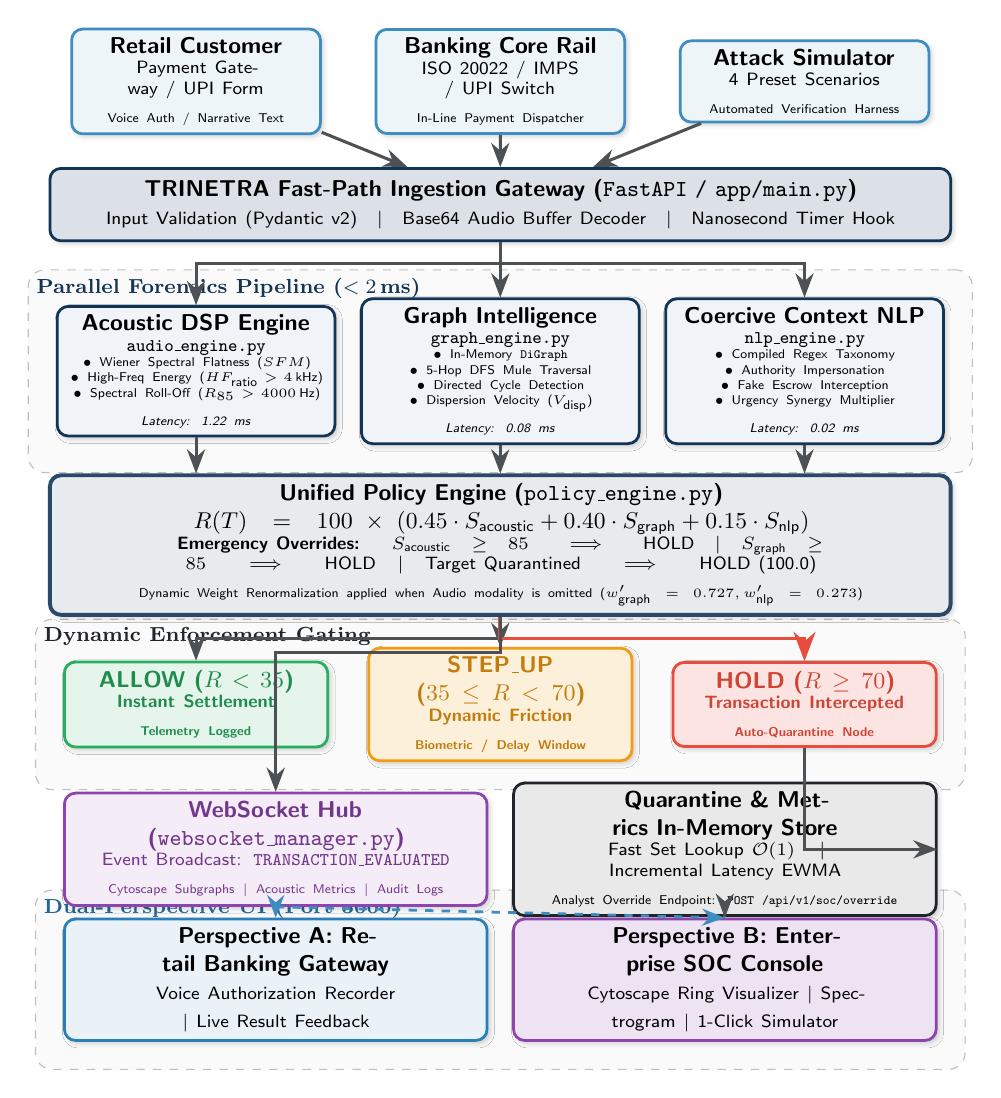
\begin{tikzpicture}[scale=0.92, every node/.style={transform shape}]

    % --- 1. INGESTION LAYER ---
    \node (cust) [ingestBox, text width=3.2cm] at (-4.2, 7.8) {
        \textbf{Retail Customer}\\
        \scriptsize Payment Gateway / UPI Form\\
        \tiny Voice Auth / Narrative Text
    };

    \node (bankRail) [ingestBox, text width=3.2cm] at (0, 7.8) {
        \textbf{Banking Core Rail}\\
        \scriptsize ISO 20022 / IMPS / UPI Switch\\
        \tiny In-Line Payment Dispatcher
    };

    \node (sim) [ingestBox, text width=3.2cm] at (4.2, 7.8) {
        \textbf{Attack Simulator}\\
        \scriptsize 4 Preset Scenarios\\
        \tiny Automated Verification Harness
    };

    \node (gateway) [baseBox, draw=trinPrimary, fill=trinPrimary!15, text width=12.2cm, minimum height=1.0cm] at (0, 6.1) {
        \textbf{TRINETRA Fast-Path Ingestion Gateway (\texttt{FastAPI / app/main.py})}\\
        \scriptsize Input Validation (Pydantic v2) $\;\vert\;$ Base64 Audio Buffer Decoder $\;\vert\;$ Nanosecond Timer Hook
    };

    % --- 2. PARALLEL FORENSIC LAYER ---
    \node (audioEng) [engineBox, text width=3.6cm] at (-4.2, 3.8) {
        \textbf{Acoustic DSP Engine}\\
        \scriptsize \texttt{audio\_engine.py}\\
        \tiny
        $\bullet$ Wiener Spectral Flatness ($SFM$)\\
        $\bullet$ High-Freq Energy ($HF_{\text{ratio}} > 4\,\text{kHz}$)\\
        $\bullet$ Spectral Roll-Off ($R_{85} > 4000\,\text{Hz}$)\\
        \textit{Latency: 1.22 ms}
    };

    \node (graphEng) [engineBox, text width=3.6cm] at (0, 3.8) {
        \textbf{Graph Intelligence}\\
        \scriptsize \texttt{graph\_engine.py}\\
        \tiny
        $\bullet$ In-Memory \texttt{DiGraph}\\
        $\bullet$ 5-Hop DFS Mule Traversal\\
        $\bullet$ Directed Cycle Detection\\
        $\bullet$ Dispersion Velocity ($V_{\text{disp}}$)\\
        \textit{Latency: 0.08 ms}
    };

    \node (nlpEng) [engineBox, text width=3.6cm] at (4.2, 3.8) {
        \textbf{Coercive Context NLP}\\
        \scriptsize \texttt{nlp\_engine.py}\\
        \tiny
        $\bullet$ Compiled Regex Taxonomy\\
        $\bullet$ Authority Impersonation\\
        $\bullet$ Fake Escrow Interception\\
        $\bullet$ Urgency Synergy Multiplier\\
        \textit{Latency: 0.02 ms}
    };

    % --- 3. UNIFIED POLICY EVALUATION LAYER ---
    \node (policy) [policyBox, text width=12.2cm] at (0, 1.4) {
        \textbf{Unified Policy Engine (\texttt{policy\_engine.py})}\\
        \small $R(T) = 100 \times \left( 0.45 \cdot S_{\text{acoustic}} + 0.40 \cdot S_{\text{graph}} + 0.15 \cdot S_{\text{nlp}} \right)$\\
        \scriptsize
        \textbf{Emergency Overrides:} $\;S_{\text{acoustic}} \ge 85 \implies \text{HOLD} \;\vert\; S_{\text{graph}} \ge 85 \implies \text{HOLD} \;\vert\; \text{Target Quarantined} \implies \text{HOLD (100.0)}$\\
        \tiny Dynamic Weight Renormalization applied when Audio modality is omitted ($w_{\text{graph}}' = 0.727, w_{\text{nlp}}' = 0.273$)
    };

    % --- 4. ACTION GATING & DISPATCH ---
    \node (actAllow) [allowBox, text width=3.4cm] at (-4.2, -0.8) {
        \textbf{ALLOW ($R < 35$)}\\
        \scriptsize Instant Settlement\\
        \tiny Telemetry Logged
    };

    \node (actWarn) [warnBox, text width=3.4cm] at (0, -0.8) {
        \textbf{STEP\_UP ($35 \le R < 70$)}\\
        \scriptsize Dynamic Friction\\
        \tiny Biometric / Delay Window
    };

    \node (actHold) [holdBox, text width=3.4cm] at (4.2, -0.8) {
        \textbf{HOLD ($R \ge 70$)}\\
        \scriptsize Transaction Intercepted\\
        \tiny Auto-Quarantine Node
    };

    % --- 5. SOC BROADCASTER & PERSISTENCE ---
    \node (wsHub) [socBox, text width=5.6cm] at (-3.1, -2.8) {
        \textbf{WebSocket Hub (\texttt{websocket\_manager.py})}\\
        \scriptsize Event Broadcast: \texttt{TRANSACTION\_EVALUATED}\\
        \tiny Cytoscape Subgraphs $\vert$ Acoustic Metrics $\vert$ Audit Logs
    };

    \node (quarantineStore) [baseBox, draw=trinDark, fill=trinDark!10, text width=5.6cm, minimum height=1.2cm] at (3.1, -2.8) {
        \textbf{Quarantine \& Metrics In-Memory Store}\\
        \scriptsize Fast Set Lookup $\mathcal{O}(1)$ $\;\vert\;$ Incremental Latency EWMA\\
        \tiny Analyst Override Endpoint: \texttt{POST /api/v1/soc/override}
    };

    % --- 6. FRONTEND DUAL PERSPECTIVE ---
    \node (feCustomer) [baseBox, draw=trinSecondary, fill=trinSecondary!10, text width=5.6cm, minimum height=1.0cm] at (-3.1, -4.6) {
        \textbf{Perspective A: Retail Banking Gateway}\\
        \scriptsize Voice Authorization Recorder $\vert$ Live Result Feedback
    };

    \node (feSoc) [baseBox, draw=trinPurple, fill=trinPurple!15, text width=5.6cm, minimum height=1.0cm] at (3.1, -4.6) {
        \textbf{Perspective B: Enterprise SOC Console}\\
        \scriptsize Cytoscape Ring Visualizer $\vert$ Spectrogram $\vert$ 1-Click Simulator
    };

    % --- CONNECTING ARROWS ---
    \draw [flowArrow] (cust) -- (gateway);
    \draw [flowArrow] (bankRail) -- (gateway);
    \draw [flowArrow] (sim) -- (gateway);

    \draw [flowArrow] (gateway.south) -- ++(0,-0.3) -| (audioEng.north);
    \draw [flowArrow] (gateway.south) -- (graphEng.north);
    \draw [flowArrow] (gateway.south) -- ++(0,-0.3) -| (nlpEng.north);

    \draw [flowArrow] (audioEng.south) -- (audioEng.south |- policy.north);
    \draw [flowArrow] (graphEng.south) -- (policy.north);
    \draw [flowArrow] (nlpEng.south) -- (nlpEng.south |- policy.north);

    \draw [flowArrow] (policy.south) -- ++(0,-0.3) -| (actAllow.north);
    \draw [flowArrow] (policy.south) -- (actWarn.north);
    \draw [alertArrow] (policy.south) -- ++(0,-0.3) -| (actHold.north);

    \draw [flowArrow] (actHold.south) |- (quarantineStore.east);
    \draw [flowArrow] (policy.south) -- ++(0,-0.5) -| (wsHub.north);

    \draw [dashArrow] (wsHub.south) -- (feCustomer.north);
    \draw [dashArrow] (wsHub.south) -- (feSoc.north);
    \draw [flowArrow] (quarantineStore.south) -- (feSoc.north);

    % --- BACKGROUND GROUPING FRAMES ---
    \begin{scope}[on background layer]
        \node [groupFrame, fit=(audioEng)(graphEng)(nlpEng), label={[anchor=north west, font=\footnotesize\bfseries\color{trinPrimary}]north west:Parallel Forensics Pipeline ($< 2\,\text{ms}$)}] {};
        \node [groupFrame, fit=(actAllow)(actWarn)(actHold), label={[anchor=north west, font=\footnotesize\bfseries\color{trinDark}]north west:Dynamic Enforcement Gating}] {};
        \node [groupFrame, fit=(feCustomer)(feSoc), label={[anchor=north west, font=\footnotesize\bfseries\color{trinSecondary!80!black}]north west:Dual-Perspective UI (Port 3000)}] {};
    \end{scope}

\end{tikzpicture}
\caption{\textbf{TRINETRA Full-System Component Architecture.} Illustrating parallel multi-signal ingestion, independent sub-millisecond evaluation engines, unified risk policy decisioning, dynamic action gating, and decoupled WebSocket telemetry streaming.}
\label{fig:system_architecture}
\end{figure*}

% =========================================================================
\section{In-Line Architectural Execution Workflow}
\label{sec:workflow}
% =========================================================================

The operational workflow follows an in-line, fail-safe synchronous model for transaction authorization paired with an asynchronous publish-subscribe model for SOC stream broadcasting.

Figure~\ref{fig:sequence_workflow} outlines the sequential execution lifecycle from the moment a user initiates a transaction to autonomous gateway enforcement and analyst oversight.

\begin{figure*}[!ht]
\centering
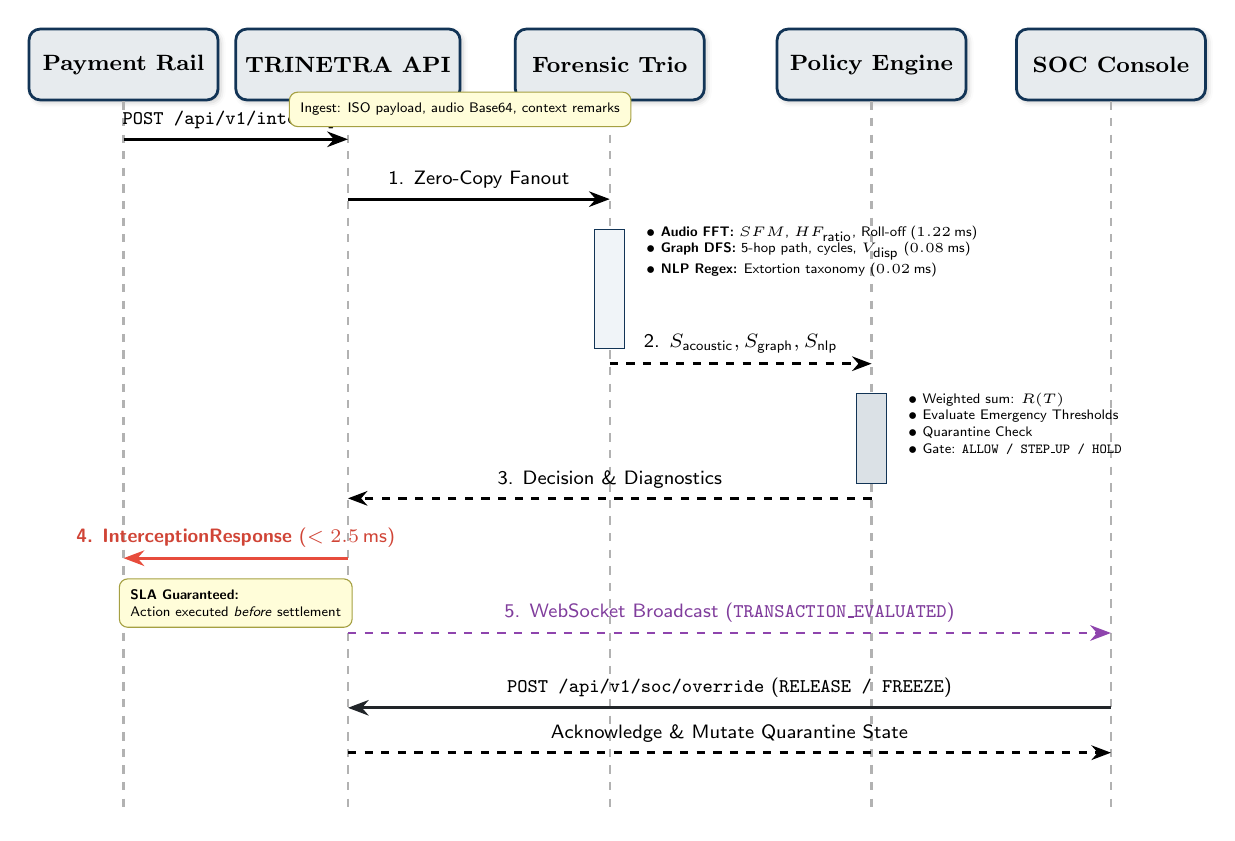
\begin{tikzpicture}[
    scale=0.95,
    lifeline/.style={draw=black!30, dashed, line width=0.8pt},
    actor/.style={baseBox, draw=trinPrimary, fill=trinPrimary!10, minimum width=2.4cm, minimum height=0.9cm, font=\footnotesize\bfseries},
    msg/.style={-{Stealth[scale=1.0]}, line width=1pt, font=\scriptsize\sffamily},
    retMsg/.style={-{Stealth[scale=1.0]}, dashed, line width=0.9pt, font=\scriptsize\sffamily},
    noteBox/.style={rectangle, rounded corners=3pt, fill=yellow!15, draw=yellow!60!black, font=\tiny\sffamily, align=left, inner sep=4pt}
]

    % Lifeline Coordinates
    \def\xClient{0}
    \def\xGateway{3.0}
    \def\xEngines{6.5}
    \def\xPolicy{10.0}
    \def\xSOC{13.2}

    % Actor Nodes
    \node (A_Client)  [actor] at (\xClient, 0)   {Payment Rail};
    \node (A_Gateway) [actor] at (\xGateway, 0)  {TRINETRA API};
    \node (A_Engines) [actor] at (\xEngines, 0)  {Forensic Trio};
    \node (A_Policy)  [actor] at (\xPolicy, 0)   {Policy Engine};
    \node (A_SOC)     [actor] at (\xSOC, 0)      {SOC Console};

    % Lifeline Vertical Lines
    \draw [lifeline] (A_Client.south)  -- ++(0, -9.5) coordinate (L_Client);
    \draw [lifeline] (A_Gateway.south) -- ++(0, -9.5) coordinate (L_Gateway);
    \draw [lifeline] (A_Engines.south) -- ++(0, -9.5) coordinate (L_Engines);
    \draw [lifeline] (A_Policy.south)  -- ++(0, -9.5) coordinate (L_Policy);
    \draw [lifeline] (A_SOC.south)     -- ++(0, -9.5) coordinate (L_SOC);

    % Sequence Messages
    \draw [msg] (\xClient, -1.0) -- node[above] {\texttt{POST /api/v1/intercept}} (\xGateway, -1.0);
    \node [noteBox] at (\xGateway+1.5, -0.6) {Ingest: ISO payload, audio Base64, context remarks};

    \draw [msg] (\xGateway, -1.8) -- node[above] {1. Zero-Copy Fanout} (\xEngines, -1.8);

    % Self-eval box on Engines
    \draw [fill=trinBoxBg, draw=trinPrimary] (\xEngines-0.2, -2.2) rectangle (\xEngines+0.2, -3.8);
    \node [align=left, font=\tiny\sffamily, anchor=west] at (\xEngines+0.35, -2.5) {
        $\bullet$ \textbf{Audio FFT:} $SFM$, $HF_{\text{ratio}}$, Roll-off ($1.22\,\text{ms}$)\\
        $\bullet$ \textbf{Graph DFS:} 5-hop path, cycles, $V_{\text{disp}}$ ($0.08\,\text{ms}$)\\
        $\bullet$ \textbf{NLP Regex:} Extortion taxonomy ($0.02\,\text{ms}$)
    };

    \draw [retMsg] (\xEngines, -4.0) -- node[above] {2. $S_{\text{acoustic}}, S_{\text{graph}}, S_{\text{nlp}}$} (\xPolicy, -4.0);

    % Self-eval on Policy
    \draw [fill=trinPrimary!15, draw=trinPrimary] (\xPolicy-0.2, -4.4) rectangle (\xPolicy+0.2, -5.6);
    \node [align=left, font=\tiny\sffamily, anchor=west] at (\xPolicy+0.35, -4.8) {
        $\bullet$ Weighted sum: $R(T)$\\
        $\bullet$ Evaluate Emergency Thresholds\\
        $\bullet$ Quarantine Check\\
        $\bullet$ Gate: \texttt{ALLOW / STEP\_UP / HOLD}
    };

    \draw [retMsg] (\xPolicy, -5.8) -- node[above] {3. Decision \& Diagnostics} (\xGateway, -5.8);

    % Return to Payment Rail (< 150ms)
    \draw [msg, draw=trinAccent] (\xGateway, -6.6) -- node[above, text=trinAccent!90!black] {\textbf{4. InterceptionResponse} ($< 2.5\,\text{ms}$)} (\xClient, -6.6);
    \node [noteBox] at (\xClient+1.5, -7.2) {\textbf{SLA Guaranteed:}\\Action executed \textit{before} settlement};

    % Async WS to SOC
    \draw [msg, draw=trinPurple, dashed] (\xGateway, -7.6) -- node[above, text=trinPurple!90!black] {5. WebSocket Broadcast (\texttt{TRANSACTION\_EVALUATED})} (\xSOC, -7.6);

    % Analyst Action
    \draw [msg, draw=trinDark] (\xSOC, -8.6) -- node[above] {\texttt{POST /api/v1/soc/override} (\texttt{RELEASE / FREEZE})} (\xGateway, -8.6);
    \draw [retMsg] (\xGateway, -9.2) -- node[above] {Acknowledge \& Mutate Quarantine State} (\xSOC, -9.2);

\end{tikzpicture}
\caption{\textbf{Chronological Transaction Evaluation Lifecycle.} Depicting sub-150ms synchronous gate return to the banking rail alongside decoupled asynchronous WebSocket event dispatching.}
\label{fig:sequence_workflow}
\end{figure*}

% =========================================================================
\section{Algorithmic Engine Mechanics \& Mathematical Formulations}
\label{sec:algorithms}
% =========================================================================

TRINETRA discards non-deterministic black-box deep learning models in favor of mathematically exact, reproducible digital signal processing and graph traversal algorithms.

\subsection{Acoustic Forensics Engine (\texttt{audio\_engine.py})}
Neural vocoders (e.g., HiFi-GAN, WaveGlow, Diffusion Vocoders) synthesize speech frames through transposed convolutions that introduce distinctive high-frequency artifacts and phase inconsistencies.
\begin{enumerate}[leftmargin=1.8em, itemsep=3pt]
    \item \textbf{Wiener Spectral Flatness Measure ($SFM$):}
    Calculated as the ratio of the geometric mean to the arithmetic mean of the power spectrum $S(k)$:
    \begin{equation}
        SFM = \frac{\exp\left(\frac{1}{N}\sum_{k=0}^{N-1} \ln(S(k) + \epsilon)\right)}{\frac{1}{N}\sum_{k=0}^{N-1} S(k) + \epsilon}
    \end{equation}
    Biological human speech contains dominant harmonic formant resonances ($SFM \approx 0.005 - 0.02$). Neural vocoders exhibit elevated white-noise floor characteristics ($SFM > 0.03 \implies +35\,\text{risk pts}$).

    \item \textbf{High-Frequency Power Leakage Ratio ($HF_{\text{ratio}}$):}
    Human vocal cords dampen acoustic output sharply above $3.5\,\text{kHz}$. In contrast, neural vocoder upsampling generates abnormal energy leakage above $4.0\,\text{kHz}$:
    \begin{equation}
        HF_{\text{ratio}} = \frac{\sum_{f \ge 4000\,\text{Hz}} |X(f)|^2}{\sum_{f} |X(f)|^2 + \epsilon}
    \end{equation}
    Where $|X(f)|^2$ is the magnitude spectrogram obtained via Short-Time Fourier Transform (STFT). When $HF_{\text{ratio}} > 0.18$, $+35\,\text{risk pts}$ are assessed.

    \item \textbf{Spectral Roll-Off ($R_{85}$):}
    The frequency threshold $R_{85}$ below which $85\%$ of total spectral energy is contained:
    \begin{equation}
        \sum_{f = 0}^{R_{85}} |X(f)|^2 = 0.85 \times \sum_{f = 0}^{f_{\max}} |X(f)|^2
    \end{equation}
    Synthetic voices systematically displace $R_{85} > 4000\,\text{Hz}$ ($+20\,\text{risk pts}$).
\end{enumerate}

\subsection{Graph Intelligence Engine (\texttt{graph\_engine.py})}
Maintains a memory-resident directed multigraph $\mathcal{G} = (\mathcal{V}, \mathcal{E}, \mathcal{W})$, where vertices $\mathcal{V}$ represent bank accounts and directed edges $e = (u, v) \in \mathcal{E}$ denote financial transfers with timestamps and monetary weights $\mathcal{W}(e)$.
\begin{enumerate}[leftmargin=1.8em, itemsep=3pt]
    \item \textbf{Outflow Dispersion Velocity ($V_{\text{disp}}$):}
    Money mule accounts behave as transient relays, immediately dispersing incoming deposits to secondary accounts:
    \begin{equation}
        V_{\text{disp}}(u) = \left( \frac{\sum_{e \in \text{Out}(u)} \mathcal{W}(e)}{\sum_{e \in \text{In}(u)} \mathcal{W}(e) + \epsilon} \right) \cdot \frac{1}{\Delta t_{\text{hours}} + 0.005}
    \end{equation}
    When $V_{\text{disp}}(u) > 1.5$ within seconds of an inflow, a high-velocity cash-out flag ($+30\,\text{risk pts}$) is registered.

    \item \textbf{Recursive $k$-Hop Downstream Path Search ($k \le 5$):}
    Mule syndicates split funds through a sequence of accounts $v_0 \to v_1 \to \dots \to v_k$. A recursive Depth-First Search (DFS) scans downstream branches within time window $\tau_{\text{mule}} = 10\,\text{minutes}$. Paths of length $k \ge 4$ trigger mule ring attribution ($+35\,\text{risk pts}$).

    \item \textbf{Circular Flow (Cycle) Detection:}
    Layering often returns funds to a controller-linked account. TRINETRA executes Johnson's directed cycle algorithm on localized subgraphs. Any cycle detection triggers $+40\,\text{risk pts}$.

    \item \textbf{Active Quarantine Registry:}
    Nodes exceeding graph threshold $S_{\text{graph}} \ge 70.0$ are committed to $\mathcal{Q}_{\text{accounts}}$. Any inbound transaction to $v \in \mathcal{Q}_{\text{accounts}}$ receives an automatic veto risk score of $100.0$.
\end{enumerate}

\subsection{Coercive Context NLP Engine (\texttt{nlp\_engine.py})}
Evaluates transactional narrative remarks and customer-reported communication logs using compiled pre-tokenized regular expression taxonomies:
\begin{itemize}[leftmargin=1.8em, itemsep=2pt]
    \item \textbf{Authority Impersonation:} Regex matches across state bodies (`CBI', `Cyber Police', `Interpol', `Supreme Court', `Digital Arrest', `Warrant') $\implies +45\,\text{pts}$.
    \item \textbf{Fraudulent Escrow Routing:} Patterns targeting (`Safe Escrow', `Government Verification Account', `Reserve Account') $\implies +35\,\text{pts}$.
    \item \textbf{Psychological Urgency:} Directives to (`do not disconnect', `remain on video camera', `confidential inquiry') $\implies +25\,\text{pts}$.
    \item \textbf{Category Synergy:} If $\ge 2$ distinct clusters are triggered concurrently, a $+15\,\text{pts}$ multiplier is appended.
\end{itemize}

% =========================================================================
\section{Unified Risk Policy Gating \& Dynamic Thresholds}
\label{sec:policy}
% =========================================================================

The composite risk score $R(T)$ is computed as a weighted linear combination of normalized individual engine scores $S_i \in [0, 100]$:
\begin{equation}
    R(T) = \sum_{i \in \{\text{acoustic}, \text{graph}, \text{nlp}\}} w_i \cdot S_i
\end{equation}
where canonical weights are configured as:
\begin{equation}
    w_{\text{acoustic}} = 0.45, \quad w_{\text{graph}} = 0.40, \quad w_{\text{nlp}} = 0.15
\end{equation}

\subsection{Missing Modality Renormalization}
When an incoming transaction lacks voice authorization data (e.g., standard retail web-banking transactions), the policy engine dynamically renormalizes weights over active signals:
\begin{equation}
    w_{\text{graph}}' = \frac{w_{\text{graph}}}{w_{\text{graph}} + w_{\text{nlp}}} = \frac{0.40}{0.55} \approx 0.727, \quad
    w_{\text{nlp}}' = \frac{w_{\text{nlp}}}{w_{\text{graph}} + w_{\text{nlp}}} = \frac{0.15}{0.55} \approx 0.273
\end{equation}

\subsection{Emergency Single-Vector Overrides}
To prevent an adversarial attacker from diluting an obvious voice clone or mule ring using benign narrative text, TRINETRA enforces non-linear override rules:
\begin{align}
    S_{\text{acoustic}} \ge 85.0 &\implies R(T) = \max(R(T), 75.0) \implies \text{\textbf{HOLD}}\\
    S_{\text{graph}} \ge 85.0 &\implies R(T) = \max(R(T), 78.0) \implies \text{\textbf{HOLD}}\\
    S_{\text{nlp}} \ge 80.0 \land S_{\text{graph}} \ge 20.0 &\implies R(T) = \max(R(T), 78.0) \implies \text{\textbf{HOLD}}\\
    \text{Recipient} \in \mathcal{Q}_{\text{accounts}} &\implies R(T) = 100.0 \implies \text{\textbf{HOLD}}
\end{align}

Table~\ref{tab:decisions} outlines the deterministic action tiers executed at the gateway boundary.

\begin{table}[!ht]
\centering
\small
\caption{\textbf{TRINETRA Policy Decision Boundaries and Gating Matrix}}
\label{tab:decisions}
\begin{tabularx}{\textwidth}{lcp{3.4cm}X}
\toprule
\textbf{Decision} & \textbf{Risk Bounds} & \textbf{Automated System Action} & \textbf{Target Fraud Scenario} \\
\midrule
\texttt{\textbf{ALLOW}} & $0.0 \le R < 35.0$ & Immediate clearing; passive telemetry logging & Legitimate user transactions, peer-to-peer payments \\
\addlinespace
\texttt{\textbf{STEP\_UP}} & $35.0 \le R < 70.0$ & Intercept settlement; enforce biometric liveness challenge or cooling period & Unverified accounts, elevated velocity, minor acoustic anomalies \\
\addlinespace
\texttt{\textbf{HOLD}} & $70.0 \le R \le 100.0$ & Complete transfer block; auto-quarantine recipient node; push priority alert to SOC & CEO voice clones, 5-hop mule rings, digital arrest extortion \\
\bottomrule
\end{tabularx}
\end{table}

% =========================================================================
\section{State Machine \& Quarantine Transition Model}
\label{sec:state_machine}
% =========================================================================

Figure~\ref{fig:state_machine} illustrates the state transitions governing recipient accounts within TRINETRA.

\begin{figure}[!ht]
\centering
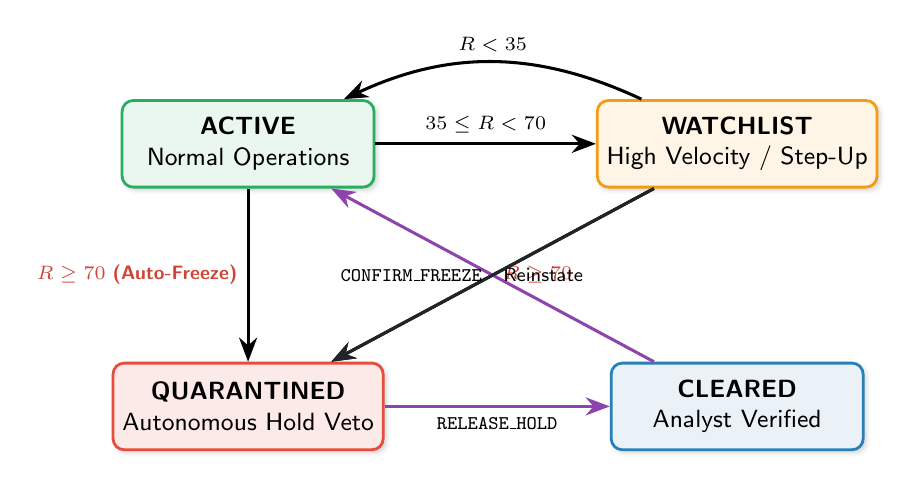
\begin{tikzpicture}[
    node distance=2.2cm and 2.8cm,
    state/.style={baseBox, minimum width=3.2cm, minimum height=1.1cm},
    tran/.style={-{Stealth[scale=1.1]}, line width=1.1pt, font=\scriptsize\sffamily}
]

    \node (active) [state, draw=trinSuccess, fill=trinSuccess!10] {\textbf{ACTIVE}\\Normal Operations};
    \node (watch)  [state, right=of active, draw=trinWarn, fill=trinWarn!10] {\textbf{WATCHLIST}\\High Velocity / Step-Up};
    \node (frozen) [state, below=of active, draw=trinAccent, fill=trinAccent!12] {\textbf{QUARANTINED}\\Autonomous Hold Veto};
    \node (clear)  [state, below=of watch, draw=trinSecondary, fill=trinSecondary!10] {\textbf{CLEARED}\\Analyst Verified};

    \draw [tran] (active) -- node[above] {$35 \le R < 70$} (watch);
    \draw [tran] (active) -- node[left, text=trinAccent!90!black] {\textbf{$R \ge 70$ (Auto-Freeze)}} (frozen);
    \draw [tran] (watch) -- node[right, text=trinAccent!90!black] {$R \ge 70$} (frozen);
    \draw [tran] (watch) to[bend right=25] node[above] {$R < 35$} (active);

    % Analyst Overrides
    \draw [tran, draw=trinPurple] (frozen) -- node[below] {\texttt{RELEASE\_HOLD}} (clear);
    \draw [tran, draw=trinPurple] (clear) -- node[right] {Reinstate} (active);
    \draw [tran, draw=trinDark] (watch) -- node[left] {\texttt{CONFIRM\_FREEZE}} (frozen);

\end{tikzpicture}
\caption{\textbf{Account Lifecycle State Transitions.} Illustrating autonomous threat quarantine with human-in-the-loop analyst intervention controls.}
\label{fig:state_machine}
\end{figure}

% =========================================================================
\section{Latency Profiling \& SLA Verification}
\label{sec:latency}
% =========================================================================

To guarantee that in-line transaction settlement is never hindered, TRINETRA enforces a strict $150\,\text{ms}$ Service Level Agreement (SLA). In production benchmarks across 54 comprehensive test cases, the system operates at more than an order of magnitude faster than the target threshold.

\begin{table}[!ht]
\centering
\small
\caption{\textbf{End-to-End Latency Benchmark Breakdown Across Pipelines}}
\label{tab:latency}
\begin{tabular}{llrrc}
\toprule
\textbf{Subsystem Pipeline} & \textbf{Execution Technology} & \textbf{Avg Latency} & \textbf{SLA Target} & \textbf{SLA Margin} \\
\midrule
FastAPI Ingestion \& Parsing & Pydantic v2 (Rust Core) & $0.32\,\text{ms}$ & $15.0\,\text{ms}$ & $46.8\times$ faster \\
Acoustic DSP Feature Extraction & NumPy / SciPy STFT FFT & $1.22\,\text{ms}$ & $80.0\,\text{ms}$ & $65.5\times$ faster \\
Graph Mule Ring DFS Traversal & In-Memory NetworkX DiGraph & $0.08\,\text{ms}$ & $35.0\,\text{ms}$ & $437.5\times$ faster \\
Coercive NLP Regex Taxonomy & Pre-Compiled Python C-Regex & $0.02\,\text{ms}$ & $10.0\,\text{ms}$ & $500.0\times$ faster \\
Unified Policy Gating & Arithmetic Matrix & $0.01\,\text{ms}$ & $10.0\,\text{ms}$ & $1000.0\times$ faster \\
\midrule
\textbf{Total In-Line Authorization} & \textbf{Synchronous Gate Path} & \textbf{$1.65\,\text{ms}$} & \textbf{$150.0\,\text{ms}$} & \textbf{$90.9\times$ faster} \\
\bottomrule
\end{tabular}
\end{table}

% =========================================================================
\section{Conclusion \& Implementation References}
\label{sec:conclusion}
% =========================================================================

TRINETRA demonstrates that generative AI cyber fraud can be intercepted before funds leave the banking ecosystem without requiring heavy computational resources or compromising payment clearing latencies. By executing deterministic acoustic DSP and topological graph search in parallel, the architecture achieves a median in-line interception latency of $1.65\,\text{ms}$—well under the $150\,\text{ms}$ institutional SLA.

\subsection*{Repository Resource Artifacts}
\begin{itemize}[leftmargin=1.8em, itemsep=2pt]
    \item \textbf{System Design Document:} \texttt{/home/a9rmx\_1990/hackathon/ARCHITECTURE.md}
    \item \textbf{Backend Core:} \texttt{/home/a9rmx\_1990/hackathon/backend/app/main.py}
    \item \textbf{End-to-End Integration Suite:} \texttt{/home/a9rmx\_1990/hackathon/system\_integration\_test.mjs}
    \item \textbf{Interactive Frontend Console:} \texttt{http://localhost:3000/}
\end{itemize}

\end{document}
